\section{Présentation d'Alter Solutions Engineering}
Alter Solutions Engineering, et plus particulièrement sa filiale Alter Frame, est l'entreprise qui m'a accueilli pour la durée de mon stage de fin d'études, nous allons donc commencer par la présenter rapidement.

\subsection{Les subdivisions d'Alter Solutions Engineering et leurs secteurs d'activité}
Alter Solutions Engineering est une entreprise relativement jeune : elle a été créée en 2006 et, si elle n'entre plus maintenant dans la catégorie des PME en termes de nombre de collaborateurs, elle reste une structure de petite taille.

Le siège social de l'entreprise se trouve à Versailles et c'est là où travaille l'équipe de développement française dont je fais partie. En pratique, il s'agit de l'équipe de développement d'Alter Frame qui est une entité enfant d'Alter Solutions Engineering (cf. section~\ref{subsec:frame}).

Alter Solutions Engineering est une société de conseil en hautes technologies mais en pratique, elle est composée de trois filières qui ont chacune une spécialité bien distinctes (cf. graphique~\ref{fig:filiales} et graphique~\ref{fig:activite}).
\begin{figure}
	\centering
	\caption{Alter Solutions Engineering et ses filiales}
	\label{fig:filiales}
	\frame{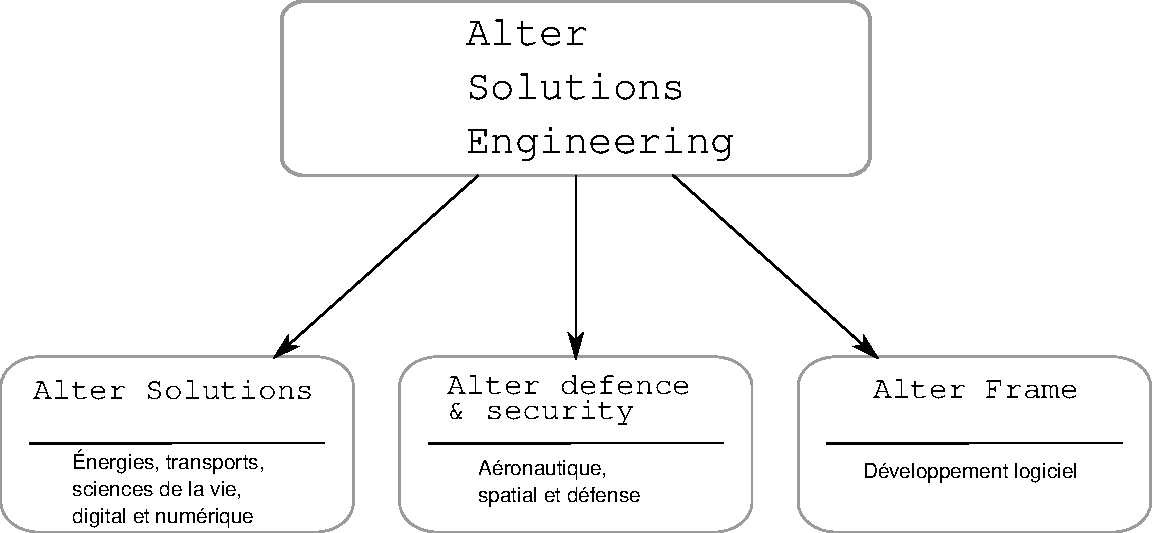
\includegraphics[width=\textwidth]{images/filiales_allinone.pdf}}
\end{figure}
\begin{figure}
	\frame{
		\begin{tikzpicture}
			\begin{axis}
				[
					axis lines*=left,
					xbar,
					xlabel={Pourcentage d'activité},
					symbolic y coords={Énergies, Aéronautique spatial et défense, Transports, Digital et numérique, Industrie, Sciences de la vie},
					ytick=data,
					xmin=0,
					xmax=50,
					nodes near coords={\pgfmathprintnumber\pgfplotspointmeta\%},
    			nodes near coords align={horizontal}
				]
				\addplot
				[
					draw=black,
					pattern=horizontal lines Purple
				]
				coordinates
				{
					(33,Énergies)
					(20,Aéronautique spatial et défense)
					(18,Transports)
					(11,Digital et numérique)
					(10,Industrie)
					(8,Sciences de la vie)
				};
			\end{axis}
		\end{tikzpicture}
		\caption{Répartition de l'activité des différentes filiales d'Alter Solutions Engineering}
		\label{fig:activite}
	}
\end{figure}
% \begin{figure}
% 	\frame{\begin{tikzpicture}
% 			\pie[color={black!80!red, black!60!purple, black!40!purple,  black!20!purple, purple!60, purple!30}, explode=0.1]{33/Énergies, 20/Aéronautique spatial et défense, 18/Transports, 11/Digital et numérique, 10/Industrie, 8/Sciences de la vie}
% 		\end{tikzpicture}}
% 	\caption{Répartition de l'activité des différentes filiales d'Alter Solutions Engineering}
% 	\label{fig:activite}
% \end{figure}

\subsubsection{Alter Solutions}
Cette filiale est spécialisée dans le conseil en ingénierie, notamment dans les domaines de l'énergie, des transports, des sciences de la vie, du digital et du numérique.

\subsubsection{Alter defence \& security}
Alter defence est également orientée vers le conseil, mais cette fois plus particulièrement dans l'aéronautique, le spatial et la défense.

Alter Defence and Security est également la filiale d'Alter Solutions Engineering qui m'accueillera une fois mon stage terminé (cf. section~\ref{sec:ccl}). L'objectif du groupe Alter au-travers de ce stage est de me donner le bagage technique et l'entraînement nécessaires pour pouvoir à terme me déployer comme expert technique auprès de clients de l'entreprise, or les missions de cyber-sécurité sont le domaine d'activité de Defence \& Security.

\subsubsection{Alter Frame}
Alter Frame enfin est la branche spécialisée dans l'édition de logiciels et celle que j'ai rejoint durant mon stage. C'est une ESN\cite{esn_wiki}\footnote{Entreprise de Services du Numérique} dont l'activité est elle-même répartie en deux catégories :
\begin{itemize}
	\item le conseil, c'est-à-dire le fait de fournir des spécialistes d'un domaine du numérique pour la durée d'un contrat à un client ;
	\item le développement de logiciels au forfait, c'est-à-dire le fait de prendre commande d'un logiciel à réaliser en interne et de le livrer à la fin du contrat.
\end{itemize}

\subsection{Un peu plus de détails sur Alter Frame}
\label{subsec:frame}
Bien qu'Alter Frame ait des clients et des domaines d'intervention variés, en termes de technologies il y a trois pôles de compétences qui sont caractéristiques de l'entreprise et reviennent le plus régulièrement :
\begin{itemize}
	\item Java ;
	\item .NET ;
	\item PHP.
\end{itemize}

Bien que mon stage se soit divisé en deux grands axes, mon travail a été dans tous les cas lié au pôle de développement Java et au responsable technique sous la direction de qui j'ai travaillé. En conséquence j'ai participé à plusieurs projets Java de manière anecdotique, en plus du projet principal que je détaillerai en partie~\ref{sec:sujet}.

Quelques projets notables d'Alter Frame, mais sur lesquels je n'ai pas eu l'occasion de travailler :
\begin{itemize}
	\item interface de \textit{monitoring} de plateformes pétrolières pour tablettes ;
	\item plateforme web permettant d'accéder facilement à des exécutables des différents projets d'Alter Frame, à destination des commerciaux des autres branches de la compagnie ;
	\item outil de vérification de conformité vis-à-vis du futur règlement européen sur la protection des données\cite{cnil}.
\end{itemize}